{%%%%%%%%%%%%%%%%%%%%%%%%%%%%%%%%%%%%%%%%%%%%%%%%%%%%%%%%%%%%%%%%%%%%%%
% 
% 	Template for Producing ASP-DAC 2013 Proceedings
% 
%%%%%%%%%%%%%%%%%%%%%%%%%%%%%%%%%%%%%%%%%%%%%%%%%%%%%%%%%%%%%%%%%%%%%%
% History
% ??/??/?? Designed by Hiroaki Kunieda (ASP-DAC '97 Publication Chair)
% 09/22/97 Modified and small bug fixed by Masaharu Imai 
% 	   (ASP-DAC '98 Publication Chair)
% 11/02/98 Modified by Tsuyoshi Isshiki
% 	   (ASP-DAC 2000 TPS Secretary)
% 7/24/00 Modified by Kiyoharu Hamaguchi
% 	   (ASP-DAC 2001 Publication chair)
% 6/18/02 Modified by Kazutoshi Kobayashi
% 	   (ASP-DAC 2003 Publication Co-Chair)
% 5/27/03 Modified by Kiyoharu Hamaguchi
% 	   (ASP-DAC 2004 TPC secretary)
% 6/10/03 Modified by Kazutoshi Kobayashi for Latex2e
% 	   (ASP-DAC 2004 Publication Co-Chair)
% 6/01/05 Modified by Nozomu Togawa
% 	   (ASP-DAC 2006 Publication Chair)
% 6/01/06 Modified by Hiroyuki Ochi
% 	   (ASP-DAC 2007 Publication Chair)
% 5/30/08 Modified by Nozomu Togawa
% 	   (ASP-DAC 2009 Publication Co-Chair)
% 4/30/10 Modified by Masashi Imai
% 	   (ASP-DAC 2011 Publication Chair)
% 3/20/12 Modified by Masashi Imai
% 	   (ASP-DAC 2013 Publication Chair)
%%%%%%%%%%%%%%%%%%%%%%%%%%%%%%%%%%%%%%%%%%%%%%%%%%%%%%%%%%%%%%%%%%%%%%
% If you have any problem, please contact ASP-DAC 2013 Publication
% Co-Chairs by E-mail at ``aspdac13publication@hal.eit.hirosaki-u.ac.jp.''
%%%%%%%%%%%%%%%%%%%%%%%%%%%%%%%%%%%%%%%%%%%%%%%%%%%%%%%%%%%%%%%%%%%%%%
%
\documentclass[twocolumn]{article}
%% If you use dvips and ps2pdf, please use Postscript font 
%% and uncomment the line below.
%%\usepackage{times}
\pagestyle{empty}
%set paper size
%for A4 paper
\topmargin      29mm    %bottom margin 30mm
\oddsidemargin  15mm    %left & right margin 15mm

%for 8 1/2" x 11" paper paper, use the following definition
%\topmargin     17mm    %bottom margin 24mm
%\oddsidemargin 18mm    %left margin 18mm & right margin 17mm

%text sizes
\textwidth  180mm
\textheight 238mm
\columnsep  5.0mm
\parindent  3.5mm

%misc parameters
\headsep 0mm  \headheight 0mm
\footskip 18mm
%\footheight 6mm

%conversion to values for LaTeX
\advance\topmargin-1in\advance\oddsidemargin-1in
\evensidemargin\oddsidemargin

\makeatletter
%as Latex considers descenders in its calculation of interline spacing,
%to get 12 point spacing for normalsize text, must set it to 10 points
\def\@normalsize{\@setsize\normalsize{12pt}\xpt\@xpt
\abovedisplayskip 10pt plus2pt minus5pt\belowdisplayskip \abovedisplayskip
\abovedisplayshortskip \z@ plus3pt\belowdisplayshortskip 6pt plus3pt
minus3pt\let\@listi\@listI}

%interline spaceing and title font for section
\def\section{\@startsection {section}{1}{\z@}{20pt plus 2pt minus 2pt}
{8pt plus 2pt minus 2pt}{\centering\normalsize\sc
\edef\@svsec{\thesection.\ }}}
\def\thesection{\Roman{section}}

%interline spacing and title font for subsection
\def\subsection{\@startsection {subsection}{2}{\z@}{16pt plus 2pt minus 2pt}
{6pt plus 2pt minus 2pt}{\normalsize\sl
\edef\@svsec{\thesubsection.\ }}}
\def\thesubsection{\Alph{subsection}}

%figures/tables captions
\long\def\@makecaption#1#2{
\vskip10pt\begin{center} #1 #2 \end{center}\par\vskip 1pt}
\def\fnum@figure{\raggedright{\footnotesize Fig. \thefigure }.%
\footnotesize}
\def\fnum@table{\footnotesize TABLE \thetable\\\footnotesize\sc}
\def\thetable{\Roman{table}}

\makeatother

%%%%%%%%%%%%%%%%%%%%%%%%%%%%%%%%%%%%%%%%%%%%%%%%%%%%%%%%%%%%%%%%%%%%%%%
\makeatletter
\newif\if@restonecol

\let\algorithm\relax
\let\endalgorithm\relax
\usepackage[tight,footnotesize]{subfigure}
\usepackage {paralist}
\usepackage{comment}
\usepackage{array}
\usepackage{amsmath}
\usepackage{graphicx}
\usepackage{amssymb}
\usepackage{url}
\usepackage[ruled]{algorithm2e}
\makeatother
\makeatletter
\providecommand{\tabularnewline}{\\}
\newtheorem{clm}{Claim}
\newtheorem{mydef}{Definition}
\newtheorem{proof}{Proof}

%%%%%%%%%%%%%%%%%%%%%%%%%%%%%%%%%%%%%%%%%%%%%%%%%%%%%%%%%%%%%%%%%%%%%%%

\begin{document}
%date not printed
\date{}

%make title
\title{\Large\textbf{On Real-Time STM Concurrency Control for Embedded Software with Improved Schedulability}}	% Modified by K. Kobayashi 18/06/02

%for single author
%\author{Center the Authors Names Here \\
%Center the Affiliations Here\\
%Center the City, Stats and Country Here\\
%{\small (it is your option if you want your entire address listed)}}

%for two authors
\begin{comment}
\author{
Mohammed Elshambakey, Binoy Ravindran\\
ECE Dept., Virginia Tech\\
Blacksburg, VA 24060, USA\\
shambake@vt.edu, binoy@vt.edu\\
}
\end{comment}

\maketitle
\thispagestyle{empty}

{\small\textbf{Abstract---
We consider software transactional memory (STM) concurrency control for embedded multicore real-time software, and present a novel contention manager for resolving transactional conflicts, called PNF. We upper bound transactional retries and task response times, and show when PNF has better schedulability than previous contention managers and lock-free synchronization. Our implementation in the Rochester STM framework/real-time Linux reveals that PNF yields comparable retry costs than competitors.}}

\section{Introduction}

Embedded systems sense physical processes and control their behavior, typically through feedback loops. Since physical processes are concurrent, computations that control them must also be concurrent, enabling them to process multiple streams of sensor input and control multiple actuators, all concurrently. Often, such computations need to concurrently read/write shared data objects. They must also process sensor input and react, while satisfying time constraints. 

Lock-based concurrency control has significant programmability, scalability, and composability challenges~\cite{Herlihy:2006:AMP:1146381.1146382}. Software transactional memory (STM) is an alternative synchronization model for shared memory data objects that promises to alleviate these difficulties. With STM, code that read/write shared objects is organized as transactions, which execute speculatively, while logging changes made to objects. Two transactions conflict if they access the same object and one access is a write. When that happens, a contention manager (CM)~\cite{Guerraoui:2005:TTT:1073814.1073863} resolves the conflict by aborting one and allowing the other to commit, yielding (the illusion of) atomicity. Aborted transactions are re-started, after rolling back the changes. In addition to a simple programming model, STM provides performance comparable to lock-free approach and is composable~\cite{Harris:2005:CMT:1065944.1065952}.  

Given STM's programmability, scalability, and composability advantages, it is a compelling concurrency control technique also for multicore embedded real-time software. However, this requires  bounding transactional  retries, as real-time threads, which subsume transactions, must satisfy time constraints.  Retry bounds under STM are dependent on the CM policy at hand.

Past real-time CM research has proposed resolving transactional contention using dynamic and fixed priorities of parent threads, resulting in Earliest Deadline First CM (ECM) and Rate Monotonic CM (RCM), respectively~\cite{6045438,stmconcurrencycontrol:emsoft11,lcmdac2012}.
In particular,~\cite{stmconcurrencycontrol:emsoft11} shows that ECM and RCM achieve higher schedulability -- i.e., greater number of task sets meeting their time constraints -- than lock-free synchronization only under some ranges for the maximum atomic section length. That range is significantly expanded with the Length-based CM (LCM) in~\cite{lcmdac2012}, increasing the coverage of STM's timeliness superiority. However, these works restrict to \textit{one} object access per transaction, which is a major limitation (Section~\ref{probelm description}). 

To allow multiple objects per transaction, we design a novel contention manager called PNF  (Section~\ref{PNF}), which can be used with global EDF (G-EDF) and global RMA (G-RMA) multicore real-time schedulers~\cite{Davis:2011:SHR:1978802.1978814}. 
We upper bound transactional retry costs and task response times (Section~\ref{rc pnf sec}). 
%, and formally compare PNF's schedulability with ECM, RCM, LCM, and lock-free synchronization (Section~\ref{sec:pnf-sched-comparison}). 
We show that PNF achieves better schedulability than lock-free synchronization for larger 
atomic section length range than ECM and RCM. Our implementation reveals that PNF yields comparable retry costs to competitors (Section~\ref{exp_eval}).

PNF's superior timeliness properties thus allow embedded real-time programmers to reap STM's significant programmability and composability advantages for a broader range of multicore embedded real-time software than what was previously possible -- paper's contribution. 

\section{Preliminaries}
\label{sec:model}

We consider a multiprocessor system with $m$ identical processors and $n$ sporadic tasks $\tau_1, \tau_2,\ldots, \tau_n$. The $k^{th}$ instance (or job) of a task $\tau_i$ is denoted $\tau_i^k$. Each task $\tau_i$ is specified by its worst case execution time (WCET) $c_i$, its minimum period $T_i$ between any two consecutive instances, and its relative deadline $D_i$, where $D_i=T_i$. Job $\tau_i^j$ is released at time $r_i^j$ and must finish no later than its absolute deadline $d_i^j=r_i^j+D_i$. Under a fixed priority scheduler such as G-RMA, $p_i$ determines $\tau_i$'s (fixed) priority and it is constant for all instances of $\tau_i$. Under a dynamic priority scheduler such as G-EDF, a job $\tau_i^j$'s priority, $p_i^j$, differs from one instance to another. 
A task $\tau_j$ may interfere with task $\tau_i$ for a number of times during an interval $L$, and this number is denoted as $G_{ij}(L)$. 


\textit{Shared objects.}
 A task may need to read/write shared, in-memory data objects while it is executing any of its atomic sections (transactions), which are synchronized using STM. 
The set of atomic sections of task $\tau_i$ is denoted $s_i$. $s_i^k$ is the $k^{th}$ atomic section of $\tau_i$. $p(s_i^k)$ is the priority of transaction $s_i^k$. Each object, $\theta$, can be accessed by multiple tasks. The set of distinct objects accessed by $\tau_i$ is $\theta_i$ without repeating objects.
The set of atomic sections used by $\tau_i$ to access $\theta$ is $s_i(\theta)$, and the sum of the lengths of those atomic sections is $len(s_i(\theta))$. $s_i^k(\theta)$ is the $k^{th}$ atomic section of $\tau_i$ that accesses $\theta$.
%
 $s_i^k$ can access one or more objects in $\theta_i$. So, $s_i^k$ refers to the transaction itself, regardless of the objects accessed by the transaction. We denote the set of all accessed objects by $s_i^k$ as $\Theta_i^k$. While $s_i^k(\theta)$ implies that $s_i^k$ accesses an object $\theta \in \Theta_i^k$, $s_i^k(\Theta)$ implies that $s_i^k$ accesses a set of objects $\Theta=\{\theta : \theta \in \Theta_i^k$ \}. $\bar{s_i^k}=\bar{s_i^k}(\Theta)$ refers only once to $s_i^k$, regardless of the number of objects in $\Theta$. So, $|\bar{s_i^k}(\Theta)|_{\forall \theta \in \Theta}=1$.
%
 $s_i^k(\theta)$  executes for a duration $len(s_i^k(\theta))$. $len(s_i^k)=len(s_i^k(\theta))=len(s_i^k(\Theta))=len(s_i^k(\Theta_i^k))$ The set of tasks sharing $\theta$ with $\tau_i$ is denoted $\gamma_i(\theta)$. Atomic sections are non-nested (supporting nested STM is future work). The maximum-length atomic section in $\tau_i$ that accesses $\theta$ is denoted $s_{i_{max}} (\theta)$, while the maximum one among all tasks is $s_{max} (\theta)$, and the maximum one among tasks with priorities lower than that of $\tau_i$ is $s_{max}^i (\theta)$.

\textit{STM retry cost.} If two or more atomic sections conflict, the CM will commit one section and abort and retry the others, increasing the time to execute the aborted sections. The increased time that an atomic section $s_i^p (\theta)$ will take to execute due to a conflict with another section $s_j^k (\theta)$, is denoted $W_{i}^{p}(s_{j}^{k}(\theta))$. If an atomic section, $s_i^p$, is already executing, and another atomic section $s_j^k$ tries to access a shared object with $s_i^p$, then $s_j^k$ is said to ``interfere" or ``conflict" with $s_i^p$. The transaction $s_j^k$ is the ``interfering transaction", and the transaction $s_i^p$ is the ``interfered transaction".

Due to \textit{transitive retry} (introduced in Section~\ref{probelm description}), an atomic section $s_i^k(\Theta_i^k)$ may retry due to another atomic section $s_j^l(\Theta_j^l)$, where $\Theta_i^k \cap \Theta_j^l = \emptyset$. $\theta_i^*$ denotes the set of objects not accessed directly by atomic sections in $\tau_i$, but can cause transactions in $\tau_i$ to retry due to transitive retry. $\theta_i^{ex}(=\theta_i + \theta_i^*)$ is the set of all objects that can cause transactions in $\tau_i$ to retry directly or through transitive retry. $\gamma_i^*$ is the set of tasks that accesses  objects in $\theta_i^*$. $\gamma_i^{ex}(=\gamma_i + \gamma_i^*)$ is the set of all tasks that can directly or indirectly (through transitive retry) cause transactions in $\tau_i$ to retry.

The total time that a task $\tau_i$'s atomic sections have to retry over $T_i$ is denoted $RC(T_i)$. The additional amount of time by which all interfering jobs of $\tau_j$ increases the response time of any job of $\tau_i$ during $L$, without considering retries due to atomic sections, is denoted $W_{ij}(L)$.

\section{Limitations of ECM, RCM, and LCM}\label{probelm description}

ECM and RCM~\cite{stmconcurrencycontrol:emsoft11} use dynamic and fixed priorities, respectively, to resolve conflicts. ECM uses G-EDF, and allows the transaction whose job has the earliest absolute deadline to commit first~\cite{6045438}. RCM uses G-RMA, and commits the transaction whose job has the shortest period.
%SH-ST
 To use STM with real-time systems, retry cost should be bounded in order to satisfy timing constraints.
%SH-END 
  Retry cost under ECM is bounded in~\cite{stmconcurrencycontrol:emsoft11} as follows:

Claim 1 (from~\cite{stmconcurrencycontrol:emsoft11}): Under ECM, a task $\tau_i$'s maximum retry cost during $T_i$ is upper bounded by:
\begin{eqnarray}
RC\left(T_{i}\right) & \le & \sum_{\theta\in\theta_{i}}\Bigg(\Big(\sum_{\tau_{j}\in\gamma_i(\theta)}\Big(\left\lceil\frac{T_{i}}{T_{j}}\right\rceil\sum_{\forall s_{j}^{l}(\theta)}len\big(s_{j}^{l}(\theta)\nonumber \\
 & + & s_{max}(\theta)\big)\Big)\Big)-s_{max}(\theta)+s_{i_{max}}(\theta)\Bigg)\label{eq3}\end{eqnarray}

%SH-ST
Retry cost under RCM is similar to ECM, except that only higher priority tasks to $\tau_i$ can interfere with any job $\tau_i^x$ of $\tau_i$. Retry cost under RCM is bounded by Claim 3 in~\cite{stmconcurrencycontrol:emsoft11}. 
%SH-END

G-EDF/LCM~\cite{lcmdac2012} and G-RMA/LCM default to ECM and RCM, respectively, with some difference. Under LCM, a higher priority transaction $s_i^k(\theta)$ cannot abort a lower priority transaction $s_j^l(\theta)$ if $s_j^l(\theta)$ has already consumed $\alpha$ percentage of its execution length. G-EDF/LCM's retry cost is bounded in~\cite{lcmdac2012} as follows:

Claim 5 (from~\cite{lcmdac2012}): $RC(T_i)$ for a task $\tau_i$ under G-EDF/LCM is upper bounded by:
\begin{eqnarray}
RC(T_i) & = & \Bigg(\sum_{\forall \tau_h \in \gamma_i}\sum_{\forall\theta \in \theta_i \wedge \theta_h}\Bigg(\left\lceil\frac{T_{i}}{T_{h}}\right\rceil\sum_{\forall s_{h}^{l}(\theta)}len\Big(s_{h}^{l}(\theta)\Big)\nonumber\\
& + & \alpha_{max}^{hl}len\Big(s_{max}^{h}(\theta)\Big)\Bigg)\Bigg)\nonumber\\
& + & \sum_{\forall s_{i}^{y}(\theta)}\Big(1-\alpha_{max}^{iy}\Big)len\Big(s_{max}^i(\theta)\Big)  
\label{eq78}\end{eqnarray} 
where $\alpha_{max}^{hl}$ is the $\alpha$ value that corresponds to $\psi$ due to the interference of $s_{max}^h(\theta)$ by $s_h^l(\theta)$. $\alpha_{max}^{iy}$ is the $\alpha$ value that corresponds to $\psi$ due to the interference of $s_{max}^i(\theta)$ by $s_i^y(\theta)$.

%SH-ST
G-RMA/LCM's retry cost is similar to G-EDF/LCM's, except that only higher priority tasks to $\tau_i$ can interfere with any job $\tau_i^x$ of $\tau_i$. G-RMA/LCM's retry cost is bounded by Claim 8 in~\cite{lcmdac2012}.
%SH-END

As mentioned before, \cite{stmconcurrencycontrol:emsoft11,lcmdac2012} assumes that each transaction accesses only one object. This assumption simplifies the retry cost (Claims 2 and 3 in~\cite{stmconcurrencycontrol:emsoft11}, and Claims 5, 8 in~\cite{lcmdac2012}) and response time analysis (Sections 4 and 5 in~\cite{stmconcurrencycontrol:emsoft11}, and Sections 4.2, 4.5 in~\cite{lcmdac2012}). Besides, it enables comparison with lock-free synchronization~\cite{key-5}. With multiple objects per transaction, ECM, RCM and LCM will face transitive retry, which we illustrate with an example.

\textbf{Example 1.} Consider three atomic sections $s_{1}^{x}$, $s_{2}^{y}$, 
and $s_{3}^{z}$ belonging to jobs $\tau_{1}^{x}$,$\tau_{2}^{y}$, 
and $\tau_{3}^{z}$, with priorities $p_{3}^{z}>p_{2}^{y}>p_{1}^{x}$, respectively. 
Assume that $s_{1}^{x}$ and $s_{2}^{y}$ share objects, $s_{2}^{y}$ and $s_{3}^{z}$
share objects. $s_{1}^{x}$ and $s_{3}^{z}$ do not share objects.
$s_{3}^{z}$ can cause $s_{2}^{y}$ to retry, which in turn will cause $s_{1}^{x}$ to retry. 
This means that $s_{1}^{x}$ may retry transitively
because of $s_{3}^{z}$, which will increase the retry cost of $s_{1}^{x}$.

Assume another atomic section $s_4^f$ is introduced. Priority of $s_4^f$ is higher than priority of $s_3^z$. $s_4^f$ shares objects only with $s_3^z$. Thus, $s_4^f$ can make $s_3^z$ to retry, which in turn will make $s_2^y$ to retry, and finally, $s_1^x$ to retry. Thus, transitive retry will move from $s_{4}^{f}$ to $s_{1}^{x}$, increasing the retry cost of $s_{1}^{x}$. 
The situation gets worse as more tasks of higher priorities are added, where each task
shares objects with its immediate lower priority task. $\tau_{3}^{z}$
may have atomic sections that share objects with $\tau_{1}^{x}$,
but this will not prevent the effect of transitive retry due to $s_{1}^{x}$.
%SH-ST
\begin{mydef}
\textbf{Transitive retry}: A transaction $s_{i}^{k}$ suffers from
transitive retry when $s_i^k$ retries due to a higher priority transaction $s_z^h$, yet $\Theta_z^h \cap \Theta_i^k=\emptyset$.
\end{mydef}
%SH-END

\begin{clm}\label{ecm-rcm-transitive-retry}
ECM, RCM and LCM suffer from transitive retry for multi-object transactions.
\end{clm}
\begin{proof}\normalfont
%SH-ST
Example 1 applies for any transactions under ECM, RCM and LCM. Claim follows.
%SH-END
\end{proof}

Therefore, the analysis in~\cite{stmconcurrencycontrol:emsoft11} and~\cite{lcmdac2012} must extend the set of objects that can cause an atomic section of a lower priority job to retry.  This can be done by initializing the set of conflicting objects, $\gamma_i$, to all objects accessed by all transactions of $\tau_i$. We then cycle through all transactions belonging to all other higher priority tasks. Each transaction $s_j^l$ that accesses at least one of the objects in $\gamma_i$ adds all other objects accessed by $s_j^l$ to $\gamma_i$. The loop over all higher priority tasks is repeated, each time with the new $\gamma_i$, until there are no more transactions accessing any object in $\gamma_i$\footnote{However, note that, this solution may over-extend the set of conflicting objects, and may even contain all objects accessed by all tasks.}.

In addition to the \emph{transitive retry} problem, retrying higher priority transactions can prevent lower priority tasks from running. This happens when all processors are busy with higher priority jobs. When a transaction retries, the processor time is wasted. Thus, it would be better to give the processor to some other task.

Essentially, what we present is a new contention manager that avoids the effect of transitive retry. We call it, Priority contention manager with Negative values and First access (or PNF). PNF also tries to enhance processor utilization. This is done by allocating processors to jobs with non-retrying transactions if any exists. PNF is described in Section \ref{PNF}.

\section{The PNF Contention Manager\label{PNF}}

Algorithm \ref{PNF-algorithm} describes PNF. It
manages two sets. The first is the $m$-set, which contains at most $m$ non-conflicting
transactions, where $m$ is the number of processors, as
there cannot be more than $m$ executing transactions (or generally,
$m$ executing jobs) at the same time. When a transaction is entered
in the $m$-set, it executes non-preemptively and no other transaction
can abort it. A transaction in the $m$-set is called an \emph{executing
transaction}. 
This means that, when a transaction is executing before
the arrival of higher priority conflicting transactions, then the
one that started executing first will be committed (Step~\ref{s_i^k commit}) (hence the term ``First access'' in the algorithm's name).

\begin{algorithm}[h]
\footnotesize{
\LinesNumbered
\KwData{
\textit{Executing Transaction:} is one that cannot be aborted by any other transaction, nor preempted by a higher priority task\;
\textit{$m$-set:} $m$-length set that contains only non-conflicting executing transactions\;
\textit{$n$-set:} $n$-length set that contains retrying transactions for $n$ tasks in non-increasing order of priority\;
\textit{n(z):} transaction at index $z$ of the $n$-set\;
$s_i^k$: a newly released transaction\;
$s_j^l$: one of the executing transactions\;
}
\KwResult{atomic sections that will commit}
\eIf{$s_i^k$ does not conflict with any executing transaction\label{s_i^k true}}
{
Assign $s_i^k$ as an executing transaction\;
Add $s_i^k$ to the $m$-set\;
Select $s_i^k$ to commit
}
{
Add $s_i^k$ to the $n$-set according to its priority\label{move to n}\;
Assign temporary priority -1 to the job that owns $s_i^k$ \label{priority to -1}\;
Select transaction(s) conflicting with $s_i^k$ for commit\label{s_i^k commit}\;
}
\If{$s_j^l$ commits\label{s_j^l commits}}
{
	\For{z=1 to size of n-set\label{traverse n-set}}
	{
		\If{n(z) does not conflict with any executing transaction\label{n(z) no conflict}}
		{
			\eIf{processor available\footnotemark \label{processor available}}
			{
				Restore priority of task owning n(z)\;
				Assign n(z) as executing transaction\;
				Add n(z) to m-set and remove it from n-set\;
				Select n(z) for commit\;
			}
			{
				Wait until processor available
			}
		}
%		move to the next n(z)\;
	}
}
}
\caption{PNF Algorithm} \label{PNF-algorithm}
\end{algorithm}
\footnotetext{An idle processor or at least one that runs a non-atomic section task with priority lower than the task holding $n(z)$.}


The second set is the $n$-set, which holds the transactions
that are retrying because of a conflict with one or more of the executing
transactions (Step~\ref{move to n}), where $n$ stands for
the number of tasks in the system. Transactions in the $n$-set are known as \emph{retrying transaction}. It also holds transactions that
cannot currently execute, because processors are busy, either due to processing executing transactions
and/or higher priority jobs. Any transaction in the $n$-set is assigned a temporal
priority of -1 (Step~\ref{priority to -1}) (hence the word 
``Negative'' in the algorithm's name). A negative priority
is considered smaller than any normal priority, and a transaction
continues to hold this negative priority until it is moved to the $m$-set, where it is restored its normal priority.


A job holding a transaction in the $n$-set can be preempted by any other job with normal priority, even if that job does not have transactions conflicting with the preempted job. Hence, this set is of length $n$, as there can be at most $n$ jobs. 
%at the same time. 
Transactions in the $n$-set whose jobs have been preempted are called preempted transactions. 
The $n$-set list keeps track of preempted transactions, because
as it will be shown, all preempted and non-preempted transactions in the $n$-set are examined when any of the
executing transaction commits. Then, one or more transactions are selected from the $n$-set to be executing transactions. If a retrying transaction is selected as an executing transaction, the task that owns the retrying transaction regains its priority.

When a new transaction is released, and if it does not conflict with
any of the executing transactions (Step~\ref{s_i^k true}), then
it will allocate a slot in the $m$-set and becomes an
executing transaction. When this transaction is released (i.e., its containing task is already allocated to a processor), it will be able to access a processor immediately. 
This transaction may have a conflict with any of the transactions in the $n$-set. However, since transactions in the $n$-set have priorities of -1, they cannot prevent this new transaction from executing if it does not conflict with any of the executing transactions.

When one of the executing transactions commits (Step~\ref{s_j^l commits}), it is time to select one of the $n$-set transactions to commit. The $n$-set is traversed from the highest priority
to the lowest priority (priority here refers to the
original priority of the transactions, and not -1) (Step~\ref{traverse n-set}).
%
If an examined transaction in the $n$-set, $s_{h}^{b}$,
does not conflict with any executing transaction (Step~\ref{n(z) no conflict}),
and there is an available processor for it (Step~\ref{processor available})
(``available'' means either an idle processor, or one that
is executing a job of lower priority than $s_{h}^{b}$),
then $s_{h}^{b}$ is moved from the $n$-set to the
$m$-set as an executing transaction and its original priority is restored. 
%
If $s_{h}^{b}$ is added to the $m$-set, the new $m$-set is compared with other transactions in the $n$-set with lower priority than $s_{h}^{b}$. 
Hence, if one of the transactions in the $n$-set, $s_{d}^{g}$, is of
lower priority than $s_{h}^{b}$ and conflicts with $s_{h}^{b}$,  
it will remain in the $n$-set. 

The choice of the new transaction
from the $n$-set depends on the original priority of transactions (hence the term  ``Priority'' in the algorithm name). The algorithm
avoids interrupting an already executing transaction to reduce its
retry cost. In the meanwhile, it tries to avoid delaying the highest priority
transaction in the $n$-set when it is time to select a new
one to commit, even if the highest priority transaction arrives after
other lower priority transactions in the $n$-set.

\subsection{Properties\label{pnf properties sec}}

\begin{clm}\label{PNF-transitive-retry}
Transactions scheduled under PNF do not suffer from transitive
retry.
\end{clm}
\begin{proof}\normalfont

%SH-ST
Proof is by contradiction. Assume three transactions $s_i^k$, $s_j^l$ and $s_z^h$. $p(s_z^h)>p(s_j^l)>p(s_i^k)$. $\Theta_i^k \cap \Theta_j^l \neq \emptyset$, $\Theta_j^l \cap \Theta_z^h \neq \emptyset$, but $\Theta_i^k \cap \Theta_z^h = \emptyset$. Assume $s_i^k$ is transitively retrying because of $s_z^h$. This means $s_i^k$, $s_j^l$ and $s_z^h$ are executing concurrently. $\Theta_i^k \cap \Theta_j^l \neq \emptyset$, so $s_i^k$ and $s_j^l$ cannot be executing transactions at the same time by definition of PNF. $\Theta_j^l \cap \Theta_z^h \neq \emptyset$, so $s_j^l$ and $s_z^h$ cannot be executing transactions at the same time by definition of PNF. Only $s_i^k$ and $s_z^h$ can be executing transactions at the same time because $\Theta_i^k \cap \Theta_z^h = \emptyset$. Hence, the three transactions cannot be running concurrently. So, $s_i^k$ cannot be transitively retrying because of $s_z^h$ which contradicts with the first assumption. Claim follows.
%SH-END
%Claim follows.
%
\end{proof}

From Claim~ \ref{PNF-transitive-retry},
%From Claims \ref{PNF-transitive-retry} and \ref{first-access},
 PNF does not increase the retry cost of multi-object transactions. However, this is not the case for ECM and RCM as shown by Claim~\ref{ecm-rcm-transitive-retry}. 

\begin{clm}\label{higher retry does not affect response}
Under PNF, any job $\tau_{i}^{x}$ is not affected by the retry cost in any other
job $\tau_{j}^{l}$.
\end{clm}
\begin{proof}\normalfont
As explained in Section~\ref{PNF-algorithm}, PNF assigns a temporary priority of -1 to any job that includes a retrying transaction. So, retrying transactions have lower priority than any other normal priority.
When $\tau_{i}^{x}$ is released and $\tau_j^l$ has a retrying transaction, $\tau_i^x$ will have a higher priority
than $\tau_j^l$. Thus, $\tau_i^x$ can run on any available processor while $\tau_j^l$ is retrying one of its transactions. Claim follows.
\end{proof}


\section{Retry Cost under PNF}\label{rc pnf sec}

We now derive an upper bound on the retry cost of any job $\tau_i^x$ under PNF during an interval $L\le T_i$. Since all tasks are sporadic (i.e., each task $\tau_i$ has a minimum period $T_i$), $T_i$ is the maximum study interval for each task $\tau_i$.

\begin{clm}\label{two transactions retry cost PNF}
%Assume two conflicting transactions $s_{i}^{k}$ and $s_{j}^{l}$.
Under PNF, the maximum retry cost suffered by a transaction $s_{i}^{k}$ due 
to a transaction $s_{j}^{l}$ is $len(s_{j}^{l})$.
\end{clm}
\begin{proof}\normalfont
By PNF's definition, $s_{i}^{k}$ cannot have started before
$s_{j}^{l}$. Otherwise, $s_i^k$ would have been an executing transaction and $s_{j}^{l}$ cannot abort it. So, the earliest release time for $s_{i}^{k}$ would have been just after $s_{j}^{l}$ starts execution. Then, $s_i^k$ would have to wait until $s_{j}^{l}$
commits. Claim follows.
\end{proof}

\begin{clm}
The retry cost for any job $\tau_{i}^{x}$ due to conflicts between its transactions and transactions of other jobs under PNF during an interval $L\le T_{i}$ is upper bounded by:
\begin{equation}
RC(L)\le\sum_{\tau_{j}\in\gamma_{i}}\left(\sum_{\theta\in\theta_{i}}\left(\left(\left\lceil \frac{L}{T_{j}}\right\rceil +1\right)\sum_{\bar{\forall s_{j}^{l}(\theta)}}len\left(\bar{s_{j}^{l}(\theta)}\right)\right)\right)\label{rc-PNF}
\end{equation}
\end{clm}

\begin{proof}\normalfont
Consider a transaction $s_{i}^{k}$ belonging to job $\tau_{i}^{x}$. By definition of PNF, higher and lower priority transactions than $s_i^k$ can become executing transaction before $s_i^k$. 
 The worst case scenario for $s_{i}^{k}$ occurs when $s_i^k$ has to wait in the $n$-set, while all other conflicting transactions with $s_i^k$ are chosen to be executing transactions. Executing transactions are not aborted. This is why $\bar{s_j^l}$ is included only once in~(\ref{rc-PNF}) for all shared objects with $s_i^k$.

The maximum number of jobs of any task $\tau_{j}$ that can interfere with $\tau_{i}^{x}$ during interval $L$ is $\left\lceil \frac{L}{T_{j}}\right\rceil +1$. From  the previous observations and Claim~\ref{two transactions retry cost PNF}, Claim follows.
\end{proof}

\begin{clm}\label{delay}
The blocking time for a job $\tau_{i}^{x}$ due to lower priority jobs 
during an interval $L\le T_{i}$ is upper bounded by:
\begin{equation}
D(\tau_{i}^{x})\le\left\lfloor \frac{1}{m}\sum_{\forall\bar{\tau_{j}^{l}}}\left(\left(\left\lceil \frac{L}{T_{j}}\right\rceil +1\right)\sum_{\forall\ddot{s_{j}^{h}}}len\left(\ddot{s_{j}^{h}}\right)\right)\right\rfloor \label{PNF-delay}
\end{equation}
where $D(\tau_{i}^{x})$ is the blocking time 
suffered by $\tau_{i}^{x}$
due to lower priority jobs. $\bar{\tau_{j}^{l}}=\{\tau_{j}^{l}:p_{j}^{l}<p_{i}^{x}\}$
and $\ddot{s_{j}^{h}}=\{s_{j}^{h}:\left(\Theta_{j}^{h} \cap \Theta_i^k = \emptyset \right) \wedge \left(\forall \Theta_i^k \in \theta_i \right)\}$. During this blocking time, all processors are unavailable for $\tau_{i}^{x}$.

\end{clm}
\begin{proof}\normalfont
Under PNF, executing transactions are non preemptive. So, a lower priority executing transaction can delay a higher priority job $\tau_i^x$ if no other processors are available. Lower priority executing transactions can be conflicting or non-conflicting with any transaction in $\tau_{i}^{x}$. If lower priority transactions are conflicting with any transaction in $\tau_i^x$, then (\ref{rc-PNF}) already covers the increase in retry cost of transactions in $\tau_i^x$ due to lower priority transactions. Otherwise, lower priority non-conflicting transactions can be executing transactions that block $\tau_i^x$.

Lower priority non-conflicting transactions can block $\tau_i^x$ when $\tau_i^x$ is newly released, or after that:

\emph{Lower priority non-conflicting transactions when $\tau_i^x$ is newly released:} $\tau_i^x$ is delayed if there are no available processors for it. Otherwise, $\tau_i^x$ can run in parallel with these non-conflicting lower priority transactions. Each lower priority non-conflicting transaction $\ddot{s_j^h}$ will delay $\tau_i^x$ for $len(\ddot{s_j^h})$.

\emph{Lower priority non-conflicting transactions after $\tau_i^x$ is released:} This situation can happen if $\tau_i^x$ is retrying one of its transactions $s_i^k$. So, $\tau_i^x$ is assigned a priority of -1. $\tau_i^x$ can be preempted by any other job. When $s_i^k$ is checked again to be an executing transaction, all processors may be busy with lower priority non-conflicting transaction and/or higher priority jobs. Otherwise, $\tau_i^x$ can run in parallel with these lower priority non-conflicting transactions.
% The effect of higher priority jobs is included by Claims~\ref{response time ecm PNF},~\ref{response rcm PNF}.

Each lower priority non-conflicting transaction $\ddot{s_j^h}$ will delay $\tau_i^x$ for $len(\ddot{s_j^h})$. From the previous cases, lower priority non-conflicting transactions act as if they were higher priority jobs interfering with $\tau_{i}^{x}$. So, the blocking time can be calculated by the interference workload given by Theorem 7 in \cite{key-2}. 
%Claim follows.
\end{proof}


\begin{clm}\label{response time ecm PNF}
%Assume that PNF is used with the G-EDF scheduler. 
The response time of a job $\tau_{i}^{x}$, during an interval $R_i^{up}\le T_{i}$, under PNF/G-EDF is upper bounded by:
\begin{equation}
R_{i}^{up}=c_{i}+RC(R_i^{up})+D_{edf}(\tau_{i}^{x})+\left\lfloor \frac{1}{m}\sum_{\forall j\ne i}W_{ij}(R_{i}^{up})\right\rfloor 
\end{equation}
where $RC(R_i^{up})$ is calculated by (\ref{rc-PNF}). $D_{edf}(\tau_{i}^{x})$
is the same as $D(\tau_{i}^{x})$ defined in~(\ref{PNF-delay}). However, for G-EDF systems. $D_{edf}(\tau_i^x)$ is calculated as:
\begin{equation}
D_{edf}(\tau_{i}^{x})\le\left\lfloor \frac{1}{m}\sum_{\forall\bar{\tau_{j}^{l}}}\begin{cases}
0 & ,R_i^{up}\le T_{i}-T_{j}\\
\sum_{\forall\ddot{s_{j}^{h}}}len\left(\ddot{s_{j}^{h}}\right) & ,R_i^{up}>T_{i}-T_{j}
\end{cases}\right\rfloor \label{d-edf}
\end{equation}
and $W_{ij}(R_{i}^{up})$ is calculated by (3) in~\cite{stmconcurrencycontrol:emsoft11}.
\end{clm}
%%%%
%%%%%%%%%%
%%%%%%%%%%%
\begin{proof}\normalfont
Response time for $\tau_{i}^{x}$ is calculated as (3) in~\cite{stmconcurrencycontrol:emsoft11} with the addition of blocking time defined by Claim \ref{delay}. G-EDF uses absolute deadlines for scheduling. This defines which jobs of the same task can be of lower priority than $\tau_{i}^{x}$, and which will not. Any instance $\tau_j^h$, released between $r_i^x - T_j$ and $d_i^x - T_j$, will be of higher priority than $\tau_i^x$. Before $r_i^x-T_j$, $\tau_j^h$ would have finished before $\tau_i^x$ is released. After $d_i^x-T_j$, $d_j^h$ would be greater than $d_i^x$. Thus, $\tau_j^h$ will be of lower priority than $\tau_i^x$. So, during $T_i$, there can be only one instance $\tau_j^h$ of $\tau_j$ with lower priority than $\tau_i^x$. $\tau_j^h$ is released between $d_i^x-T_j$ and $d_i^x$. Consequently, during $R_i^{up}<T_i-T_j$, no existing instance of $\tau_j$ is of lower  priority than $\tau_i^x$. Hence, 0 is used in the first case of~(\ref{d-edf}). But if $R_i^{up}>T_i-T_j$, there can be only one instance $\tau_j^h$ of $\tau_j$ with lower priority than $\tau_i^x$. Hence, $\left\lceil\frac{R_i^{up}}{T_i}\right\rceil+1$ in~(\ref{PNF-delay}) is replaced with 1 in the second case in~(\ref{d-edf}). Claim follows.
\end{proof}


\begin{clm}\label{response rcm PNF}
%Assume that PNF is used with the G-RMA scheduler. 
The response time of a job $\tau_{i}^{x}$, during an interval $R_i^{up}\le T_{i}$, under PNF/G-RMA is upper bounded by: 
\begin{equation}
R_{i}^{up}=c_{i}+RC(R_i^{up})+D(\tau_{i}^{x})+\left\lfloor \frac{1}{m}\sum_{\forall j\ne i,p_j>p_i}W_{ij}(R_{i}^{up})\right\rfloor 
\end{equation}
where $RC(L)$ is calculated by (\ref{rc-PNF}), $D(\tau_{i}^{x})$
is calculated by (\ref{PNF-delay}), and $W_{ij}(R_{i}^{up})$
is calculated by (2) in~\cite{stmconcurrencycontrol:emsoft11}.
\end{clm}
\begin{proof}\normalfont
Proof is same as of Claim \ref{response time ecm PNF}, 
except that G-RMA assigns fixed priorities. Hence, (\ref{PNF-delay}) can be used directly for calculating $D(\tau_{i}^{x})$ without modifications. Claim follows.
\end{proof}


%%%
\section{Experimental Evaluation}\label{exp_eval}

%Having established PNF's retry and response time bounds, and the conditions under which it outperforms ECM, RCM, LCM, and lock-free synchronization, 
We now would like to understand how PNF's retry cost compares with competitors in practice (i.e., on average). Since this can only be understood experimentally, we implement PNF and the competitors and conduct experiments. 

%\subsection{Experimental Setup}

We used the ChronOS real-time Linux kernel~\cite{dellinger2011chronos}
and the RSTM library~\cite{marathe2006lowering} in our implementation. We implemented G-EDF and G-RMA schedulers in ChronOS, and modified RSTM to include implementations of ECM, RCM, LCM, and PNF. For the retry-loop lock-free synchronization, we used a loop that reads an object and attempts to write to it  using a CAS  instruction. The task retries until the CAS succeeds. We used an 8 core, 2GHz AMD Opteron platform. The average time taken for one write operation by RSTM on any core is 0.0129653375$\mu s$, and the average time taken by one CAS-loop operation on any core is 0.0292546250 $\mu s$.

We used four task sets consisting of 4, 5, 8, and 20 periodic tasks. Each task runs in its own thread and has a set of atomic sections. Atomic section properties are probabilistically controlled using three parameters: the maximum and minimum lengths of any atomic section within a task, and the total length of atomic sections within any task. Since lock-free synchronization cannot handle more than one object per atomic section, we first compare PNF's retry cost with that of lock-free (and other CMs) for one object per transaction. We then compare PNF's retry cost with that of other CMs for multiple objects per transaction.

%SH-ST
Figure
%~\ref{fig:pnf_results_uniobject} and
~\ref{fig-RC-pnf-4t} shows the average retry cost for the 
%5 task and 
4 task case
%, respectively,
 under 
% 1 and 
 5 shared objects.
% , respectively. 
On the x-axis of the figures, we record 3 parameters $x$, $y$, and $z$. $x$ is the ratio of the total length of all atomic sections of a task to the task WCET. $y$ is the ratio of the maximum length of any atomic section of a task to the task WCET. $z$ is the ratio of the minimum length of any atomic section of a task to the task WCET. Confidence level of all data points is 0.95. 

From Figure~\ref{fig-RC-pnf-4t}, we observe that PNF has shorter or comparable retry cost than ECM, RCM, and LCM. Similar trends were observed for the other task sets. Those are omitted here for brevity.
%, and are available in~\cite{stmconcurrencycontrol_techreport}.
%SH-END

\begin{figure}[h]
\centering
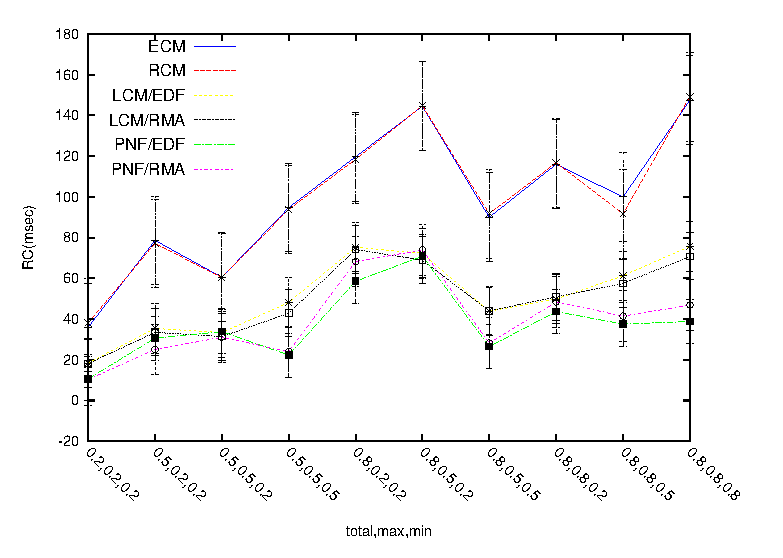
\includegraphics[scale=0.5]{figures/Abr_dur_4t_5obj_1wr}
\caption{Avg. retry cost (5 shared objects, 4 tasks).}
\label{fig-RC-pnf-4t}
\end{figure}



\section{Conclusions}\label{conclusion}

Transitive retry increases transactional retry cost under ECM, RCM, and LCM. PNF avoids transitive retry by avoiding   transactional preemptions. PNF reduces the priority of aborted transactions to enable other tasks to execute, increasing processor usage. Executing transactions are not preempted due to the release of higher priority jobs. On the negative side of PNF, higher priority jobs can be blocked by executing transactions of lower priority jobs. 

\bibliographystyle{abbrv}
%\small{\bibliography{global_bibliography}}
\footnotesize{\bibliography{global_bibliography}}



\end{document}
